
%\documentclass[xcolor=pdftex,dvipsnames,table]{beamer}
\documentclass[xcolor=pdftex,dvipsnames,table]{beamer}

\usetheme{Amsterdam}

\usefonttheme[onlymath]{serif}
\setbeamertemplate{navigation symbols}{}
\setbeamertemplate{footline}[frame number]

\usepackage{animate}
\usepackage{lmodern}
\usepackage{comment}
\usepackage{natbib}
\usepackage{graphicx}
%\usepackage{pgf}
\usepackage{pbox}
\usepackage{pifont}
\usepackage{alltt}
\usepackage{verbatim}
\usepackage{multirow}
\usepackage{xspace}
\usepackage{cases}
\usepackage{geometry}
%\usepackage{tikz}
%\usetikzlibrary{arrows,automata,positioning}
%\usepackage[absolute,overlay]{textpos}
\usepackage[normalem]{ulem}
%\usepackage{tikz-qtree}
\usepackage{pbox}
%\usepackage{ragged2e}
%\usepackage{pifont}

%\usepackage[all]{xy}

\usepackage{latexsym}
\usepackage{amsmath}
\usepackage{amssymb}
\usepackage{xfrac}

\usepackage{notation}
\usepackage{variables}
\usepackage{drawing}
%\usepackage{xparse}
%\usepackage{tikz}
%\usetikzlibrary{calc}



\newcommand{\dquote}[1]{``{#1}''}
\newcommand{\squote}[1]{`{#1}'}
\newcommand{\pgivenbf}[3]{${#1}(\mathbf{#2} | \mathbf{#3})$}
\newcommand{\pgiven}[3]{${#1}({#2} | {#3})$}
\newcommand{\pofbf}[2]{${#1}(\mathbf{#2})$}
\newcommand{\pof}[2]{${#1}({#2})$}
\newcommand{\indice}[1]{$_{#1}$}
\newcommand{\cgray}[1]{\textcolor{gray}{{#1}}}
\newcommand{\cblue}[1]{\textcolor{blue}{{#1}}}
\newcommand{\cred}[1]{\textcolor{red}{{#1}}}
\newcommand{\coran}[1]{\textcolor{Orange}{{#1}}}
\newcommand{\cgreen}[1]{\textcolor{Green}{{#1}}}
\newcommand{\cellbl}{\cellcolor{black}}
\newcommand{\cellblue}{\cellcolor{blue}}
\newcommand{\cellgreen}{\cellcolor{green}}
\newcommand{\cellr}{\cellcolor{red}}
\newcommand{\cellg}{\cellcolor{gray}}
\newcommand{\celldg}{\cellcolor{darkgray}}
\newcommand{\lra}{$\leftrightarrow$}
\newcommand{\WX}{\textcolor{white}{X}}
\newcommand{\WDot}{\textcolor{white}{$\cdot$}}
\newcommand{\WN}[1]{\textcolor{white}{#1}}
\newcommand{\vtext}[1]{\begin{sideways}#1\end{sideways}}
\newcommand{\phr}[1]{$\overset{\_}{#1}$}
\newcommand{\phs}{\overset{\_}{s}}
\newcommand{\pht}{\overset{\_}{t}}
\newcommand{\hypoe}[2]{\fbox{$\overset{\text{#1}}{#2}$}}
\newcommand{\hypot}[2]{\fbox{$\overset{\text{#1}}{\text{#2}}$}}
%\newcommand{\argmax}{\operatornamewithlimits{argmax}}
%\newcommand{\thickbar}[1]{\mathbf{\bar{\text{$#1$}}}}



% declares a document
\begin{document}



	%\title{Employee's social media use}
	%\title{Social media use by employees}
	\title{NMT project}
	%\subtitle{for unsupervised language learning}

	%\author{Miguel Rios}
	\institute[UvA]{
		%\inst{1}
		Universiteit van Amsterdam\\
	}

	\date{\today}
	
	% Title page
	{\setbeamertemplate{footline}{}
	\begin{frame}[plain]
		\titlepage
	\end{frame}
	}


	% Table of contents	
	%\frame[allowframebreaks]{
	{\setbeamertemplate{footline}{}
	\begin{frame}
		\frametitle{Content}
		\tableofcontents
	\end{frame}
	}



	% trick to start counting from the table of contents
	\setcounter{framenumber}{0}


	% SLIDES
	\section{Seq2seq}
	\begin{frame}{NMT}

	%Argument {10} sets the desired frame rate (frames per second), {0} and {214} set the first and last file numbers of the PNG series to be included in the animation.
   \animategraphics[loop,autoplay,width=\linewidth]{10}{seq2seq_gif/seq2seq-}{0}{214}

	\end{frame}
	
	\begin{frame}{NMT}
	\begin{figure}
	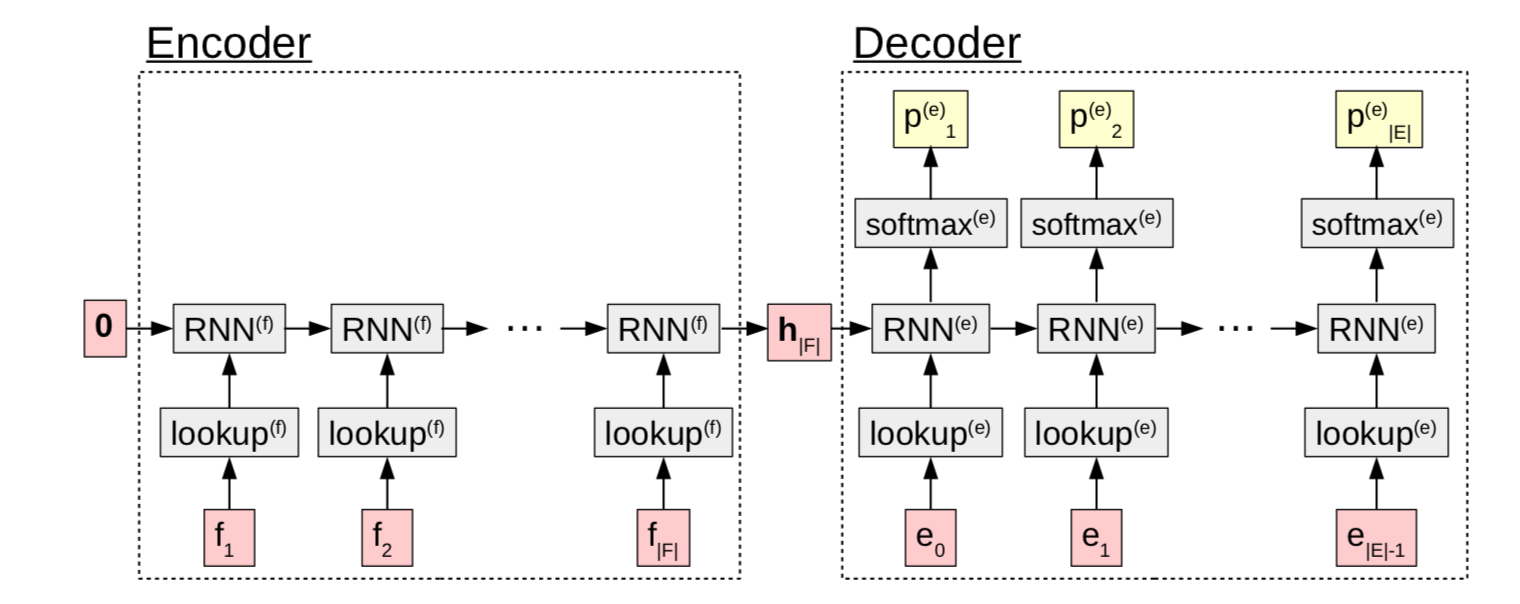
\includegraphics[scale=0.45]{img/encdec}

	\end{figure}
	\end{frame}
	
	\begin{frame}{seq2seq}
	\textbf{Homework}
	\begin{itemize}
	\item Neural Machine Translation and Sequence-to-sequence Models: A Tutorial
	\begin{itemize}
	\item \textbf{Section 5.1 - 5.3} Neural Networks and Feed-forward Language Models
	\item \textbf{Section 6.1-6.4, 6.5} Recurrent Neural Network Language Models
	\end{itemize}
	\item Familiarise with preprocessing (Tokenizer, Lowercase, BPE)
	\end{itemize}
	\end{frame}
	
	\newcounter{finalframe}
	\setcounter{finalframe}{\value{framenumber}}
	
	
	{\setbeamertemplate{footline}{}
    \begin{frame}[plain]{Questions?}
    \end{frame}
  	}
	
	%\section*{References}
	
	%\input{backup}


	%\frame[allowframebreaks]{ \frametitle{References}
       % \bibliographystyle{plainnat}
        %\bibliography{../bib}
	%}

	

	% Trick to discount regular frames from the total of backup frames
	\setcounter{framenumber}{\value{finalframe}}
	
	
\end{document}
